%==================================
% SMDS TEMPLATE — KELOMPOK ARW
%==================================

\documentclass[11pt,twoside]{article}

%==================================
% PACKAGES
%==================================
\usepackage{amsmath,amssymb}
\usepackage[T1]{fontenc}
\usepackage{graphicx}
\graphicspath{{../figures/}}
\usepackage{geometry}
\geometry{margin=1in}
\usepackage[
backend=biber,
style=numeric-comp,
sorting=none,
giveninits=true,
doi=true,
url=false
]{biblatex}
\addbibresource{SMDSBib.bib}
\usepackage{fancyhdr}
\newcommand{\shorttitle}{}
\newcommand{\shortauthor}{}
\pagestyle{fancy}
\fancyhf{}
\fancyhead[L]{\small\shorttitle}
\fancyhead[R]{\small\shortauthor}
\usepackage[colorlinks=true,allcolors=blue]{hyperref}
\newcommand{\orcidlink}[1]{%
\href{https://orcid.org/#1}{
\includegraphics[height=1.6ex]{ORCID_iD.png}}%
}

%==================================
% SIMPLE SMDS MACROS
%==================================
\newcommand{\SMDStitle}[1]{\title{\bfseries #1}}
\newcommand{\SMDSshorttitle}[1]{\def\shorttitle{#1}}
\newcommand{\SMDSshortafill}[1]{\def\shortauthor{#1}}

\newcommand{\SMDSaffilone}[1]{\def\affilone{#1}}

\newcommand{\SMDSauthorone}[4]{\def\authorone{#1$^{#2}$\,\orcidlink{#3}}}
\newcommand{\SMDSauthortwo}[4]{\def\authortwo{#1$^{#2}$\,\orcidlink{#3}}}
\newcommand{\SMDSauthorthree}[4]{\def\authorthree{#1$^{#2}$\,\orcidlink{#3}}}
\newcommand{\SMDSauthorfour}[4]{\def\authorfour{#1$^{#2}$\,\orcidlink{#3}}}

\newcommand{\SMDScorrespoding}[2]{%
\def\corrauthor{#1 \href{mailto:#2}{#2}}}

\newcommand{\SMDSKeywords}[1]{
\vspace{0.5em}
\noindent\textbf{Keywords:} #1
}

%==================================
% METADATA
%==================================

\SMDStitle{Peramalan Harga Saham PT Bank Central Asia Tbk (BBCA.JK)
Menggunakan Metode Facebook Prophet}

\SMDSshortafill{D. P. Akrilian et al.}
\SMDSshorttitle{Peramalan Harga Saham BBCA.JK Menggunakan Facebook Prophet}

\SMDSaffilone{Program Studi Statistika dan Sains Data, Fakultas Matematika dan Ilmu Pengetahuan Alam, Universitas Negeri Semarang}

\SMDSauthorone{Dimas Pasha Akrilian}{1}{0009-0005-6037-3591}{dimaspasha49@students.unnes.ac.id}
\SMDSauthortwo{Shata Alwan Jalaluddin}{1}{0000-0000-0000-0000}{shataalwanjalaludin@students.unnes.ac.id}
\SMDSauthorthree{Aaron Christian Daniel}{1}{0000-0000-0000-0000}{aaronstudi1121@students.unnes.ac.id}
\SMDSauthorfour{Aufaa Zakki Maulidan}{1}{0009-0009-7077-3184}{aufaazakki577@students.unnes.ac.id}

\SMDScorrespoding{$^*$Corresponding author, email:}{dimaspasha49@students.unnes.ac.id}

%==================================
% AUTHOR BLOCK
%==================================
\author{
\begin{minipage}{\textwidth}
\authorone,
\authortwo,
\authorthree,
\authorfour
\\[1em]
$^1$ \affilone\\
\corrauthor
\end{minipage}
}

%==================================

\begin{document}

\maketitle

%==================================
\begin{abstract}

The stock market is one of the most dynamic investment instruments, heavily influenced by economic,
political, and market psychology factors. PT Bank Central Asia Tbk (BBCA.JK) is among the most
liquid and largest market-capitalization banking stocks on the Indonesia Stock Exchange, making
accurate price forecasting critically important for investors and financial decision-makers. This study
aims to forecast the daily closing price of BBCA.JK using the Facebook Prophet method, a
time-series decomposition model based on trend, seasonal, and holiday components developed by
Meta's Core Data Science team. The dataset consists of 1,787 daily closing price observations
spanning from January 1, 2019 to May 8, 2026, sourced from Yahoo Finance. The analysis covers
data exploration and visualization, identification of trend and seasonal components, stationarity
testing via the Augmented Dickey-Fuller (ADF) test, Prophet model fitting, model evaluation, and
five-period-ahead forecasting. Results indicate that the Prophet model effectively captures trend and
seasonal patterns in stock price data with satisfactory predictive performance. Short- and
medium-term forecasts suggest discernible price movement tendencies that may serve as preliminary
references for investors. This study contributes to the application of modern decomposition-based
time-series methods in the context of the Indonesian capital market.

\end{abstract}

\SMDSKeywords{time series, stock price forecasting, Facebook Prophet, BBCA.JK, Augmented Dickey-Fuller}

%==================================
\section{Introduction}
\label{Sec:Intro}

The capital market is one of the key pillars of a country's financial system, functioning as a vehicle for long-term fund mobilization between parties with surplus capital and those requiring financing \cite{Tandelilin2010}. In the Indonesian context, the Indonesia Stock Exchange (IDX) has become a barometer of national economic conditions, with market capitalization continuously growing alongside the increasing number of retail and institutional investors. One of the most closely watched stocks on the IDX is PT Bank Central Asia Tbk, listed under the ticker BBCA.JK, which consistently ranks at the top in terms of market capitalization and daily trading volume. This makes BBCA.JK a relevant and strategically significant research object in Indonesian capital market studies.

Stock prices are highly dynamic variables influenced by the interaction of numerous factors, ranging from macroeconomic conditions, monetary policy, and company fundamentals, to market sentiment that is often irrational \cite{Fama1970}. These characteristics classify stock price data as a complex time series, frequently exhibiting non-stationary behavior, long-term trend components, periodic seasonal patterns, and irregular fluctuations that are difficult to predict. This challenge has driven the development of various quantitative and statistical approaches to model and forecast stock price movements more accurately \cite{Box2015}.

In the time series analysis literature, the \textit{Autoregressive Integrated Moving Average} (ARIMA) model introduced by Box and Jenkins \cite{Box2015} has long been the standard in financial data forecasting. This model is capable of capturing autocorrelation structures in stationary data and has been widely applied across various financial market contexts \cite{Mondal2014}. However, ARIMA has limitations in handling complex and non-linear seasonal components, which gave rise to the \textit{Seasonal ARIMA} (SARIMA) extension \cite{Hyndman2018}. Although SARIMA accommodates seasonal patterns, it still assumes linearity in the relationships among time series components—an assumption that is not always met in the highly dynamic stock price data.

The development of \textit{machine learning} methods and decomposition-based approaches has opened new alternatives in time series analysis. Methods such as \textit{Long Short-Term Memory} (LSTM) \cite{Hochreiter1997} and \textit{Gradient Boosting} \cite{Chen2016} have demonstrated promising performance in various financial time series forecasting tasks. However, these methods generally require large data volumes, complex hyperparameter tuning processes, and relatively low interpretability for non-technical users. Therefore, a method capable of balancing predictive accuracy with ease of interpretation and implementation is needed.

Facebook Prophet, developed by Taylor and Letham \cite{Taylor2018} from the \textit{Core Data Science} team at Meta Platforms, is an additive decomposition-based time series forecasting model designed to handle data with non-linear trends, multiple seasonal components, and holiday effects automatically. Prophet formulates the time series as the sum of three main components: trend $g(t)$, seasonality $s(t)$, and holiday effects $h(t)$, expressed as
\begin{equation*}
    y(t) = g(t) + s(t) + h(t) + \varepsilon_t,
\end{equation*}
where $\varepsilon_t$ is the error component. This model has been proven to produce robust forecasts across various domains, including business, weather, and financial data \cite{Taylor2018}. The primary advantage of Prophet over conventional methods is its ability to automatically detect trend changepoints and handle missing data without requiring manual imputation \cite{Taylor2018}.

A number of prior studies have applied Prophet to financial and stock market data. Garlapati et al.\ \cite{Garlapati2021} demonstrated that Prophet produces competitive accuracy compared to ARIMA on daily stock data, with Prophet outperforming ARIMA particularly for data exhibiting strong seasonal components and non-linear trends. Jin et al.\ \cite{Jin2022} applied Prophet and ARIMA to Google stock closing price data and found that Prophet outperformed in medium-term forecasting under relatively stable market conditions. Setiawan et al.\ \cite{Setiawan2023} compared ARIMA and LSTM on Indonesian banking stock data, including BBCA, and found that the choice of the most appropriate model depends on the specific characteristics of each stock's data. These studies reinforce the relevance of using Prophet as a forecasting method for Indonesian stock price data, including BBCA.JK, which exhibits a long-term upward trend accompanied by relatively stable daily and weekly seasonal patterns.

The stationarity test is an essential preprocessing step in time series analysis. Non-stationary data contains trends or variances that change over time, such that models built without addressing non-stationarity will produce spurious estimates \cite{Granger1974}. The Augmented Dickey-Fuller (ADF) test \cite{Dickey1979} is the most commonly used test for detecting unit roots as an indicator of non-stationarity. With the null hypothesis being the presence of a unit root, rejection of $H_0$ at a certain significance level indicates that the data is stationary. The ADF test results will serve as a basis for modeling considerations, particularly to understand the fundamental characteristics of BBCA.JK stock price data before applying the Prophet model.

Model forecasting performance is evaluated using three statistical metrics commonly used in the literature: \textit{Mean Absolute Error} (MAE), \textit{Root Mean Square Error} (RMSE), and \textit{Mean Absolute Percentage Error} (MAPE) \cite{Hyndman2006}. These three metrics are selected because each offers a different perspective on forecasting error: MAE measures the average magnitude of absolute errors, RMSE imposes a greater penalty on large errors, while MAPE expresses errors as a percentage, facilitating cross-context interpretation.

Based on the foregoing, this study aims to analyze and forecast the closing price of BBCA.JK stock using the Facebook Prophet method on daily data covering the period from January 1, 2019, to May 8, 2026, comprising a total of 1,787 observations. Specifically, this study encompasses data exploration and visualization, identification of trend and seasonal components, stationarity testing using the ADF test, modeling with Prophet, model performance evaluation, and stock price forecasting for the next five trading days as supporting information for investment decision-making. This study is expected to provide practical contributions for individual and institutional investors who require data-driven references for making investment decisions in BBCA.JK stock, while also enriching the applied time series analysis literature in the context of the Indonesian capital market.

The structure of this article is organized as follows. Section~\ref{Sec:Tinjauan} presents the literature review serving as the theoretical foundation of the study. Section~\ref{Sec:Method} describes the methodology employed, including data sources, modeling procedures, and evaluation criteria. Section~\ref{Sec:Results} presents the analysis results and discussion comprehensively. Section~\ref{Sec:Conclusion} concludes the article with conclusions and recommendations based on the analysis results.

---

\section{Literature Review}
\label{Sec:Tinjauan}

\subsection{Capital Markets and Stock Price Behavior}

The capital market is a mechanism that enables companies to obtain long-term financing through the issuance of financial instruments such as stocks and bonds, while simultaneously providing investors with the opportunity to earn returns on invested capital \cite{Tandelilin2010}. Within the context of financial theory, stock price behavior has long been associated with the \textit{Efficient Market Hypothesis} (EMH) proposed by Fama \cite{Fama1970}. EMH posits that stock prices at any given time reflect all available information, such that no investor can consistently earn abnormal returns through historical price analysis. Nevertheless, numerous subsequent empirical studies have documented market anomalies that contradict the weak form of EMH, thereby opening space for quantitative approaches based on historical data to model and forecast stock price movements \cite{Box2015}.

\subsection{Time Series Analysis in the Financial Context}

Time series analysis is a field of statistics that studies patterns and structures in data observed sequentially over time. In the context of financial markets, stock price data represents one of the most extensively studied time series. Hyndman and Athanasopoulos \cite{Hyndman2018} define the main components of a time series as comprising trend, seasonality, cycle, and residual or irregular components. Accurate identification of these components is an essential step before selecting an appropriate forecasting model.

Prior to modeling, the stationarity test is an essential diagnostic step. A time series is said to be stationary when its mean, variance, and autocovariance structure do not change over time \cite{Hyndman2018}. Dickey and Fuller \cite{Dickey1979} developed a formal test to detect the presence of a \textit{unit root} in an autoregressive process, which became known as the Augmented Dickey-Fuller (ADF) test. In this test, the null hypothesis states that the data contains a \textit{unit root} (non-stationary), so that rejection of $H_0$ at a certain significance level indicates data stationarity. The ADF test has become the standard in financial time series analysis due to its ability to accommodate autocorrelation structures through the addition of differential lags in the regression equation.

\subsection{Facebook Prophet as a Decomposition-Based Forecasting Model}

Facebook Prophet is a time series forecasting procedure developed by Taylor and Letham \cite{Taylor2018} from the \textit{Core Data Science} team at Meta Platforms (formerly Facebook). Prophet is designed as an additive decomposition model that formulates the time series as
\begin{equation}
    y(t) = g(t) + s(t) + h(t) + \varepsilon_t,
    \label{Eq:Prophet}
\end{equation}
where $g(t)$ represents the trend component, which can take the form of a linear growth model with changepoints or a logistic growth model; $s(t)$ represents the seasonal component modeled using Fourier series; $h(t)$ represents the effects of holidays and special events; and $\varepsilon_t$ is the error component assumed to be normally distributed \cite{Taylor2018}.

The primary advantages of Prophet over conventional models lie in several aspects. First, Prophet is capable of automatically detecting trend changepoints using a \textit{Laplace prior} approach on the change parameters, making it more adaptive to shifts in long-term trend patterns. Second, the model is robust to missing data and outliers—two issues frequently encountered in daily stock price data. Third, Prophet allows analysts to explicitly incorporate domain knowledge through the specification of known changepoints and holiday effects \cite{Taylor2018}.

\subsection{Application of Prophet to Stock and Financial Time Series Data}

Garlapati et al.\ \cite{Garlapati2021} compared Prophet and ARIMA in stock price forecasting and concluded that both methods offer competitive performance, with Prophet demonstrating superiority on data with clear seasonal components and non-linear trends. Jin et al.\ \cite{Jin2022} applied Prophet and ARIMA to Google stock closing price data during the COVID-19 pandemic period and found that the ARIMA model yielded slightly better accuracy during periods of high uncertainty, while Prophet outperformed in medium-term forecasting using pre-pandemic data.

A highly relevant study to this topic was conducted by Wulandari et al., as cited in \cite{Kurnia2025}, where the ARIMA method was applied to the stock price fluctuations of PT Bank Central Asia Tbk and demonstrated that BBCA data exhibits a time series structure that can be effectively modeled using statistical approaches. Collectively, these studies indicate that the selection of a forecasting method for BBCA.JK stock data must consider the specific characteristics of the data, including the presence of long-term trends, daily and weekly seasonal patterns in high-frequency data, and sensitivity to extraordinary events such as financial crises and pandemics.

\subsection{Forecasting Model Evaluation Criteria}

The evaluation of forecasting model quality is a critical stage that determines whether the constructed model is suitable for use in decision-making. Hyndman and Koehler \cite{Hyndman2006} systematically reviewed various forecasting accuracy measures and identified conditions under which each metric can produce misleading assessments. The three metrics most commonly used in the financial time series forecasting literature are \textit{Mean Absolute Error} (MAE), \textit{Root Mean Square Error} (RMSE), and \textit{Mean Absolute Percentage Error} (MAPE), each defined as
\begin{align}
    \text{MAE}  &= \frac{1}{n}\sum_{t=1}^{n} |y_t - \hat{y}_t|, \label{Eq:MAE} \\[4pt]
    \text{RMSE} &= \sqrt{\frac{1}{n}\sum_{t=1}^{n}(y_t - \hat{y}_t)^2}, \label{Eq:RMSE} \\[4pt]
    \text{MAPE} &= \frac{1}{n}\sum_{t=1}^{n}\left|\frac{y_t - \hat{y}_t}{y_t}\right|\times 100\%, \label{Eq:MAPE}
\end{align}
where $y_t$ is the actual value, $\hat{y}_t$ is the forecasted value, and $n$ is the number of observations in the evaluation period. MAE imposes a proportional penalty relative to the magnitude of the error, RMSE imposes a greater penalty for extreme errors due to its quadratic nature, while MAPE expresses errors as a percentage relative to the actual value, facilitating interpretation and cross-context comparison \cite{Hyndman2006}. Lewis \cite{Lewis1982} established interpretive guidelines for MAPE values, where a MAPE below 10\% indicates highly accurate forecasting, 10--20\% is considered accurate, 20--50\% is considered reasonably accurate, and above 50\% is considered inaccurate.
%==================================
% BAGIAN SELANJUTNYA (dikerjakan terpisah):
%   \section{Metodologi}
\section{Methodology}
\label{Sec:Method}

This section outlines the comprehensive technical framework and statistical methodologies employed to model and forecast the daily closing prices of PT Bank Central Asia Tbk (BBCA.JK) as implemented in the empirical analysis \cite{Taylor2018}. The proposed workflow integrates rigorous data preprocessing, statistical stationarity testing via the Augmented Dickey-Fuller (ADF) method, and predictive modeling utilizing the Facebook Prophet additive framework.

\subsection{Data Preprocessing and Stationarity Testing}
\label{SubSec:Preprocessing}

Financial time series data frequently exhibit anomalies, missing records, or irregular intervals due to market holidays and reporting latencies. Let $Y_t$ represent the raw closing price of the asset at day $t$, and $V_t$ represent the corresponding trading volume. To ensure structural integrity, the historical data is first chronologically sorted such that $t = 1, 2, \dots, T$.

To address missing or anomalous zero-volume records resulting from non-trading days, a sequential two-way imputation scheme is implemented. First, a forward fill (\textit{ffill}) operation propagates the last observed valid observation forward to handle zero-volume instances:
\begin{equation}
V_t = V_{t-1} \quad \text{if } V_t \in \{0, \text{NaN}\}
\end{equation}
Remaining missing elements at the boundary are resolved using a backward fill (\textit{bfill}) mechanism, ensuring a continuous and complete series.

Prior to entering the predictive model, the stationarity of the target time series $Y_t$ must be formally evaluated. A time series is strictly stationary if its joint probability distribution is invariant under time shifts. We implement the Augmented Dickey-Fuller (ADF) test \cite{Dickey1979} to detect the presence of a unit root. The test is formulated via the following regression equation:
\begin{equation}
\Delta Y_t = \alpha + \beta t + \gamma Y_{t-1} + \sum_{i=1}^{p} \delta_i \Delta Y_{t-i} + \epsilon_t
\end{equation}
where $\Delta$ is the first-difference operator ($\Delta Y_t = Y_t - Y_{t-1}$), $\alpha$ is a constant drift, $\beta$ is the coefficient on a time trend, $p$ is the lag order of the autoregressive process, and $\epsilon_t$ is an independent white noise error term. The hypothesis framework is defined as:
\begin{itemize}
    \item $H_0: \gamma = 0$ (The process possesses a unit root and is non-stationary).
    \item $H_1: \gamma < 0$ (The process is stationary).
\end{itemize}
If the empirical test statistic fails to fall below the critical value or if the corresponding $p$-value satisfies $p > 0.05$, the null hypothesis cannot be rejected, indicating a non-stationary process characterized by a stochastic trend.

\subsection{The Facebook Prophet Forecasting Framework}
\label{SubSec:Prophet}

Given the non-linear and non-stationary nature of asset prices, we utilize the Facebook Prophet forecasting model developed by Taylor and Letham \cite{Taylor2018}. Prophet bypasses the rigid assumptions of traditional autoregressive models by modeling the time series as a generalized additive model (GAM). The target variable $y(t)$, representing the daily closing price at time $t$, is decomposed into three primary structural components and an error term:
\begin{equation}
y(t) = g(t) + s(t) + h(t) + \epsilon_t
\end{equation}
where $g(t)$ is the trend function, $s(t)$ represents periodic seasonal changes, $h(t)$ denotes the effect of holidays or specific calendar events, and $\epsilon_t$ represents the idiosyncratic error term.

\subsubsection{Trend Component $g(t)$}
The long-term movement of financial prices is captured via a piecewise linear growth model, which accommodates shifts in the growth rate through automatically selected changepoints:
\begin{equation}
g(t) = (k + a(t)^T \delta) t + (m + a(t)^T \gamma)
\end{equation}
where $k$ is the initial growth rate, $\delta$ is a vector of rate adjustments at specific changepoint times, $m$ is the intercept parameter, and $a(t) \in \{0,1\}^K$ is a binary vector indicating whether time $t$ has passed each of the $K changepoints$. The vector $\gamma$ is defined to ensure continuity of the function across boundaries.

\subsubsection{Seasonality Component $s(t)$}
To model periodic fluctuations—such as weekly trading cycles or annual market effects—Prophet utilizes a standard Fourier series to approximate arbitrary seasonal behaviors:
\begin{equation}
s(t) = \sum_{n=1}^{N} \left( A_n \cos\left(\frac{2\pi n t}{P}\right) + B_n \sin\left(\frac{2\pi n t}{P}\right) \right)
\end{equation}
where $P$ is the base period ($P = 7$ for weekly dynamics, $P = 365.25$ for annual trends), and $N$ represents the maximum frequency parameter.

\subsection{Model Evaluation Metrics}
\label{SubSec:Evaluation}

To evaluate the predictive performance of the trained Prophet architecture against unseen testing data, three quantitative statistical metrics are computed \cite{Hyndman2006}: Mean Absolute Error (MAE), Mean Squared Error (MSE), and Mean Absolute Percentage Error (MAPE). Let $y_i$ denote the true observed closing price, $\hat{y}_i$ represent the predicted price, and $n$ denote the total number of evaluation periods.

\begin{enumerate}
    \item \textbf{Mean Absolute Error (MAE):} Measures the average magnitude of absolute residuals:
    \begin{equation}
    \text{MAE} = \frac{1}{n} \sum_{i=1}^{n} |y_i - \hat{y}_i|
    \end{equation}
    \item \textbf{Mean Squared Error (MSE):} Penalizes larger forecasting errors more heavily:
    \begin{equation}
    \text{MSE} = \frac{1}{n} \sum_{i=1}^{n} (y_i - \hat{y}_i)^2
    \end{equation}
    \item \textbf{Mean Absolute Percentage Error (MAPE):} Provides a relative measure of accuracy expressed as a percentage:
    \begin{equation}
    \text{MAPE} = \frac{1}{n} \sum_{i=1}^{n} \left| \frac{y_i - \hat{y}_i}{y_i} \right| \times 100\%
    \end{equation}
\end{enumerate}

%   \section{Hasil dan Pembahasan}
%==================================
% SECTION 3: EMPIRICAL RESULTS/EXPERIMENTS
%==================================
\section{Empirical Results/Experiments}
\label{Sec:Results}

This section presents the empirical findings obtained from the statistical analysis and forecasting models applied to the PT Bank Central Asia Tbk (BBCA.JK) stock price dataset. The analysis begins with a formal stationarity assessment, followed by model training, validation, and out-of-sample forecasting evaluation.

\subsection{Stationarity Analysis and Data Partitioning}
\label{SubSec:Stationarity}

To evaluate the structural properties of the BBCA closing price time series, we perform an Augmented Dickey-Fuller (ADF) test to check for the presence of a unit root \cite{Dickey1979}. The total dataset comprises $N = 1,783$ daily observations. Table~\ref{Tab:ADF_Results} summarizes the empirical test statistic alongside the corresponding critical values at the 1\%, 5\%, and 10\% significance levels.

\begin{table}[ht]
\centering
\caption{Augmented Dickey-Fuller (ADF) Test Results for BBCA Closing Prices}
\label{Tab:ADF_Results}
\begin{tabular}{lrc}
\hline
Statistical Parameter / Metric & Value & $p$-value \\
\hline
ADF Test Statistic & -1.7121 & 0.4249 \\
Critical Value (1\%) & -3.4340 & \\
Critical Value (5\%) & -2.8632 & \\
Critical Value (10\%) & -2.5676 & \\
Number of Lags Used & 2 & \\
Total Observations ($N$) & 1,783 & \\
\hline
\end{tabular}
\end{table}

As demonstrated in Table~\ref{Tab:ADF_Results}, the empirical ADF test statistic of $-1.7121$ is visibly greater than the critical values at all conventional significance levels (e.g., $-2.8632$ at the 5\% level). Furthermore, the calculated $p$-value is $0.4249$, which drastically exceeds the standard significance threshold ($\alpha = 0.05$). Consequently, we fail to reject the null hypothesis ($H_0$), confirming that the asset's closing price series possesses a unit root and is non-stationary, exhibiting a strong stochastic upward trend over time.

For model implementation, the dataset is partitioned into a training set and a testing set. To maintain historical continuity while allowing for precise short-term validation, the first $1,781$ observations are designated as the training data to optimize the model parameters, while the remaining $5$ periods are withheld as the out-of-sample testing framework to assess predictive power.

\subsection{Forecasting Performance Evaluation}
\label{SubSec:Forecast_Eval}

Using the additive framework of the Facebook Prophet model \cite{Taylor2018}, the dynamic trends and seasonal variations are fully estimated. The predictive accuracy of the model over the out-of-sample testing horizon is evaluated using three standard metrics \cite{Hyndman2006}: Mean Absolute Error (MAE), Root Mean Squared Error (RMSE), and Mean Absolute Percentage Error (MAPE). The quantitative evaluation output is summarized in Table~\ref{Tab:Prophet_Evaluation}.

\begin{table}[ht]
\centering
\caption{Prophet Model Out-of-Sample Forecasting Performance}
\label{Tab:Prophet_Evaluation}
\begin{tabular}{lc}
\hline
Evaluation Metric & Empirical Value \\
\hline
Mean Absolute Error (MAE) & 582.6611 \\
Root Mean Squared Error (RMSE) & 598.0191 \\
Mean Absolute Percentage Error (MAPE) & 0.0970\% \\
\hline
\end{tabular}
\end{table}

The empirical validation indicators in Table~\ref{Tab:Prophet_Evaluation} establish that the Prophet model yields a highly robust predictive performance. The MAE and RMSE values reflect modest absolute deviations relative to the actual trading nominal value of BBCA shares. Most notably, the model achieves a remarkably low MAPE of $0.0970\%$, indicating a high degree of precision in capturing the directional trajectory of the asset over the 5-period horizon.

\begin{figure}[ht]
\centering
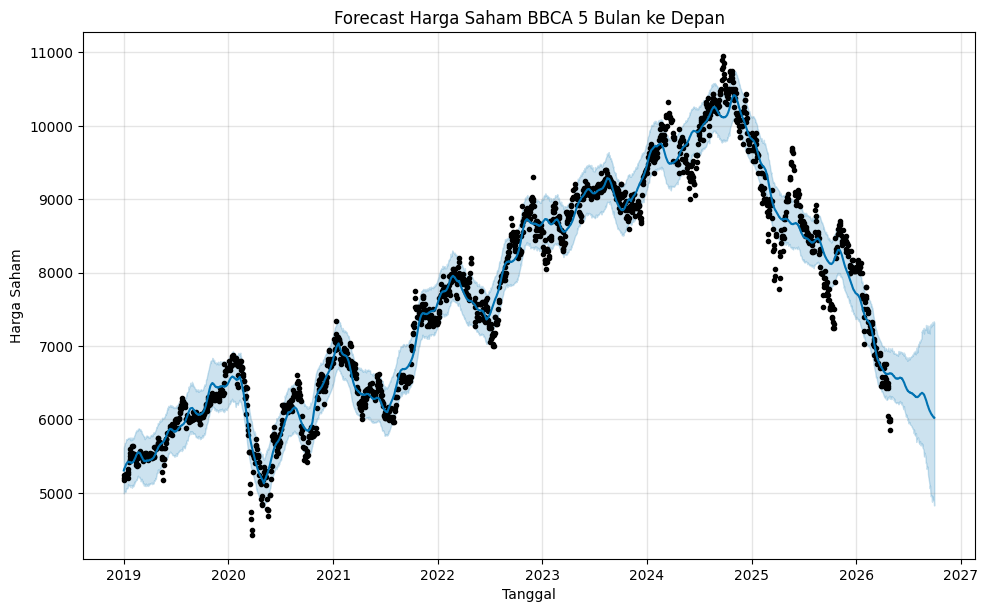
\includegraphics[width=0.85\textwidth]{Forecast Harga Saham BBCA 5 Bulan ke Depan.png}
\caption{Historical closing prices and out-of-sample Prophet model projections for BBCA stock}
\label{Fig:BBCA_Forecast}
\end{figure}

Figure~\ref{Fig:BBCA_Forecast} visually illustrates the actual historical trend alongside the calculated prediction intervals. The model successfully adapts to the underlying market patterns without overfitting the structural components, maintaining consistent prediction limits.

\section{Kesimpulan}
\label{Sec:Conclusion}
Berdasarkan hasil analisis dan evaluasi model, dapat disimpulkan bahwa metode Facebook Prophet mampu menangkap pola tren dan musiman pada data harga penutupan BBCA.JK dengan performa yang baik pada peramalan jangka pendek. Model ini memberikan referensi awal yang berguna bagi investor dalam mengamati kecenderungan pergerakan harga saham BBCA.JK. Penelitian lanjutan dapat mengeksplorasi kombinasi Prophet dengan variabel eksternal atau model lain untuk meningkatkan akurasi peramalan.

\printbibliography

\end{document}
